\documentclass[]{article}

% Package
\usepackage{amsmath}
\usepackage{breqn}
\usepackage[english]{babel}
\usepackage{graphicx}
\usepackage{float}
\usepackage{subcaption}
\usepackage{booktabs}
%\graphicspath{figures/}

%opening
\title{SC4045: Deformable Mirror}
\author{Yudha Prawira Pane - 4321499}

\begin{document}

\maketitle

\begin{abstract}
This report explains the basic theory and implementation of deformable mirror as a wavefront corrector in adaptive optics. The deformable mirror is modeled after Keck Observatory Telescope. To quantify the accuracy of the wavefront constructed by the mirror, its approximation power is calculated. This measure is then repeated for different number of actuators. 
\end{abstract}

\section{Constructing H Matrix}
The $ H $ matrix is constructed by calculating the influence function $ S(x,y) $ for each of its element. The function is formulated as follows:
\begin{dmath}
S(x,y) = \left\lbrace \frac{w_1}{2\pi \sigma^2_1}exp\left[\frac{-((x-x_{act}[i])^2 + (x-y_{act}[i])^2)}{2\sigma^2_1} \right]  +  \frac{w_2}{2\pi \sigma^2_2}exp\left[\frac{-((x-x_{act}[i])^2 + (x-y_{act}[i])^2)}{2\sigma^2_2} \right] \right\rbrace 0.470 \mu m
\end{dmath}

$ x_{act}[i] $ and $ y_{act}[i] $ is $ x $ and $ y $ coordinate of $ i $-th actuator. This function basically looks like a 2D gaussian distribution whose mean is the position of the actuators (assuming position as a point) and variance are $ \sigma_1 $ and $ \sigma_2 $. To get an insight about the mirror's shape, Figure \ref{fig1}  is what the mirror looks like when one of the actuators is "poked".

\begin{figure}[H]
\centering
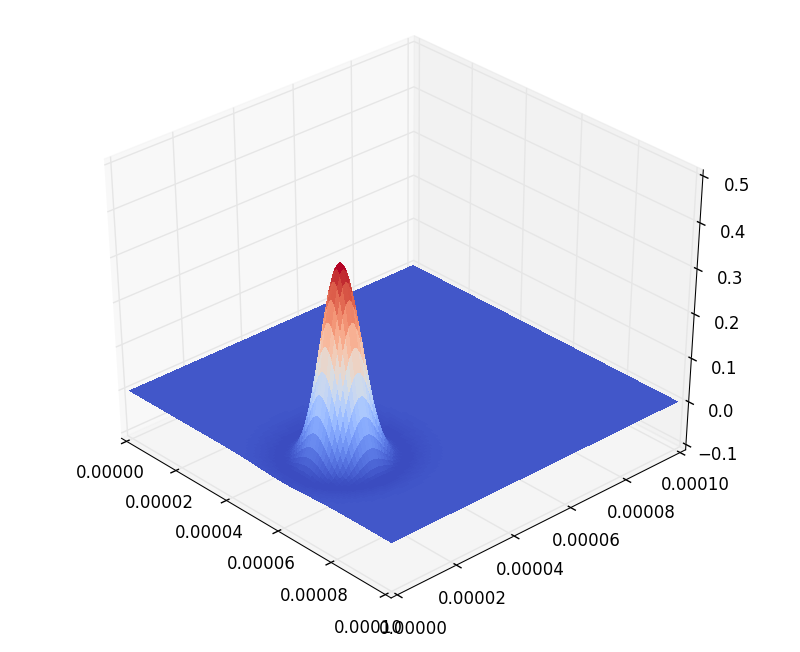
\includegraphics[width=0.4\linewidth]{figures/poke}
\caption{Mirror shape when one actuator is "poked'}
\label{fig1}
\end{figure}

\section{Estimating the Best Actuators Input}
The deformable mirror's phase $ \phi_{\text{DM}} $ and actuator inputs $ u $ is related according the following equation:

\begin{equation}
\phi_{\text{DM}} = Hu
\label{eqdm}
\end{equation}

where $ \phi_{\text{DM}} \in \mathcal{R}^m $, $ u = \in \mathcal{R}^n $, $ H \in \mathcal{R}^{mxn} $ and $ m>n $.

Now, given an estimated $ \hat{\phi} $ from the wavefront reconstruction, calculate $u$ that best approximates this wavefront using linear least square principle.

\begin{equation}
u = (H^\top H)^{-1}H^\top \hat{\phi}
\end{equation}


Afterwards, \eqref{eqdm} is used once again to obtain $ \phi_{\text{DM}} $.

\section{Implementation}

\subsection{Approximation power comparison}
To demonstrate that the method above indeed works, the deformable mirror is implemented with following assumptions. 

\begin{enumerate}
\item Mirror shape: rectangular
\item Number of lenslet : 25
\item Number of wavefront samples $ N_{\phi} $: 36 
\item Wavefront-lenslet configuratio: hudgin geometry
\item Distance between $ \phi $ samples: 8.46 $ \mu $m
\item Wavefront generator: random function   with $ \mu $ = 0.5 and $ \sigma $ = 0.001.
\end{enumerate}

Based on above configuration, the actuators and wavefront samples are positioned as in Figure \ref{mirror_config}. As we can see, this positioning is implemented according to hudgin geometry [2].


\begin{figure}[h!]
\centering
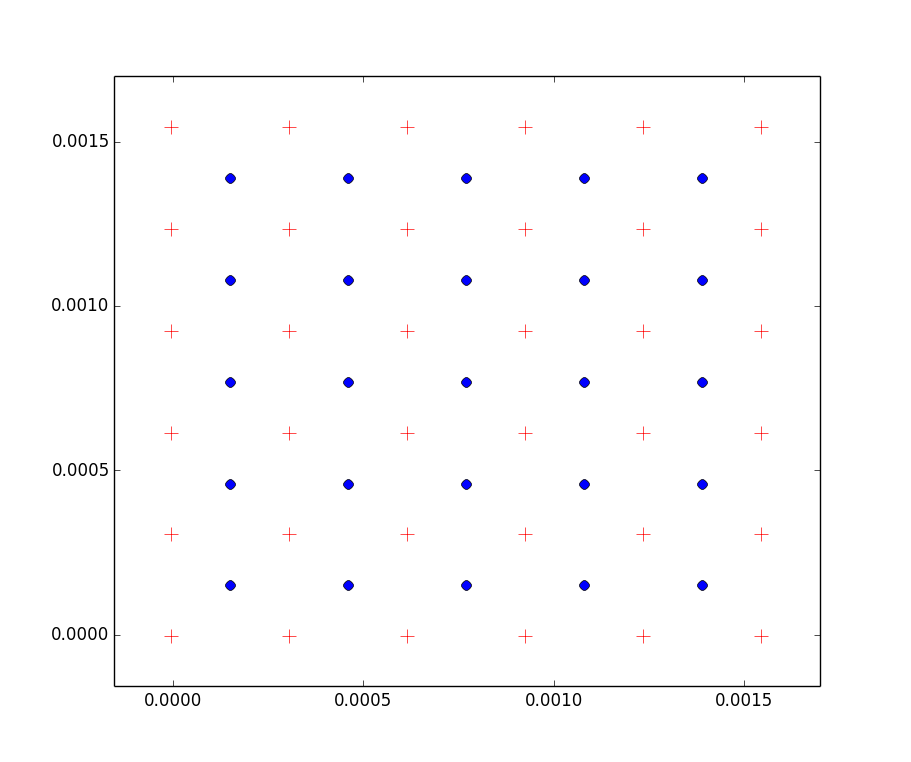
\includegraphics[width=0.7\linewidth]{figures/mirror_config}
\caption{Position of actuators (blue) and wavefront samples (red)}.
\label{mirror_config}
\end{figure}

The optimal estimate for the actuators input according to least square sense is then calculated. Subsequently, this value is used to calculate $ \phi_{\text{DM}} $. The comparison of $ \hat{\phi} $ surface  with  $ \phi_{\text{DM}} $ surface is shown in Figure \ref{fig:surf}. Visually, we are tempted to say that the deformable mirror manages to reconstruct the wavefront quite well. However, for a more quantitative measure, one can use approximation power of the surface. This approximation power is implemented as root-mean square of the wavefront error \eqref{rms}. Applying this measure, we obtain the error to be $ 6.3423\times10^{-5} $. This value is relatively low with respect to the generated wavefront magnitude. 

\begin{equation}
e_{RMS} = \frac{1}{N}\sqrt{\sum_{i=1}^{N} (\hat{\phi}_i  - \phi_{\text{DM}_i})^2} \quad \text{$ N $ = number of wavefront samples}
\label{rms}
\end{equation}

\begin{figure}[h!]
        \centering
        \begin{subfigure}[b]{0.5\textwidth}
                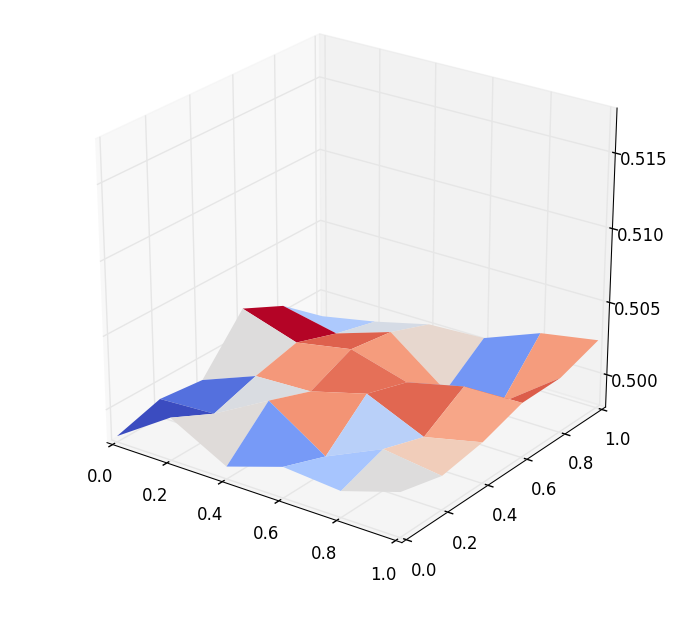
\includegraphics[width=\textwidth]{figures/surf_phi_hat}
                \caption{Surface of reconstructed wavefront}
                \label{fig:surf_phi_hat}
        \end{subfigure}%
        ~ %add desired spacing between images, e. g. ~, \quad, \qquad, \hfill etc.
          %(or a blank line to force the subfigure onto a new line)
        \begin{subfigure}[b]{0.6\textwidth}
                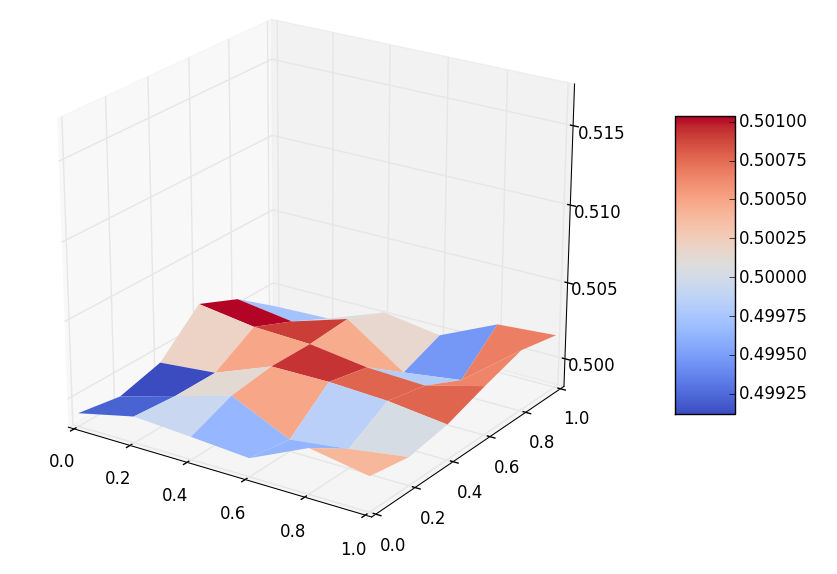
\includegraphics[width=\textwidth]{figures/surf_phi_dm}
                \caption{Surface of deformable mirror}
                \label{fig:surf_phi_dm}
        \end{subfigure}
        \caption{Reconstructed wavefront surface}
        \label{fig:surf}
\end{figure}



\subsection{The influence of the number of actuators}
It is of an interest to observe the influence of number of actuators in terms of approximating power. In order to do this, a fix number of wavefront is used ($ N_{\phi} = 256$). We vary the number of actuators but still adhering to rectangular configuration. However, is also important to note that once the number of actuators is no longer sufficient to form a hudgin geometry, they are arranged such that they covers the entire mirror in equal distance. For instance, 5$ \times $5 and 9$ \times $9 actuators would be positioned as in Figure \ref{fig:mirror_configs}.

\begin{figure}[h!]
        \centering
        \begin{subfigure}[b]{0.4\textwidth}
                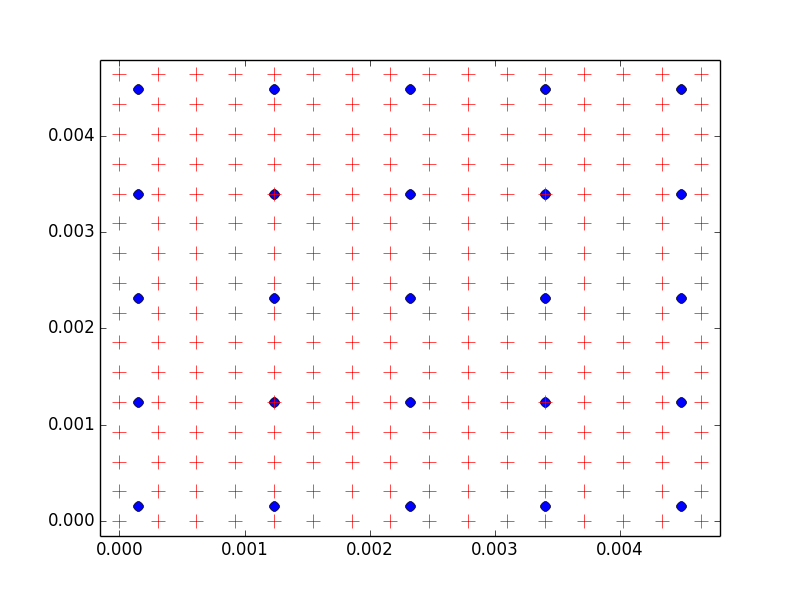
\includegraphics[width=\textwidth]{figures/mirror_config5}
                \label{fig:mirror_config5}
        \end{subfigure}%
        ~ %add desired spacing between images, e. g. ~, \quad, \qquad, \hfill etc.
          %(or a blank line to force the subfigure onto a new line)
        \begin{subfigure}[b]{0.4\textwidth}
                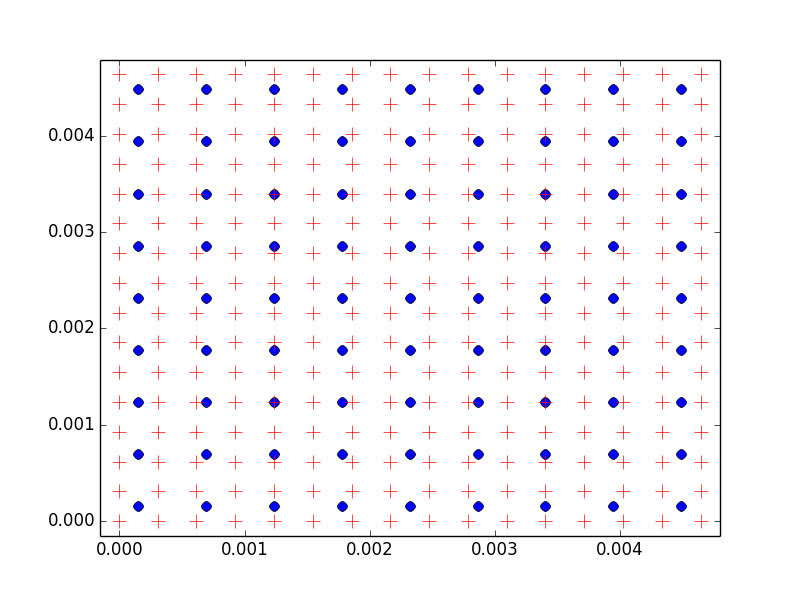
\includegraphics[width=\textwidth]{figures/mirror_config9}
                \label{fig:mirror_config9}
        \end{subfigure}
        \caption{Positioning for 5$\times$5 and 9$\times$9 actuators}
        \label{fig:mirror_configs}
\end{figure}

Unsurprisingly, we obtain increasing magnitude of error with decreasing number of actuators. This magnitude is listed in Table \ref{tab:act}. As we can see, the accuracy drastically decrease when the number of actuator is decreased from 225 to 169. This in part due to the error introduced in the pseudo inverse calculation. To visualize this influence, Figure \ref{approx_power} shows the interpolated curve of accuracy with respect to number of actuators.

\begin{table}[h!]
\centering
\caption{Subgradient Inequality Comparison for J}  
    \label{tab:act}
    \begin{tabular}{c|c}
        \toprule
        Number of actuators & error RMS\\
        \midrule        
        $ 9 $ & 0.4728 \\
        $ 25 $ &  0.4420 \\
        $ 49 $ &  0.3732 \\
        $ 81 $ &  0.2120 \\
        $ 121 $ & 0.0581 \\
        $ 169 $ & 0.0537 \\
		$ 225 $ & 0.0003624 \\
		$ 289 $ & 1.3072$ \times $ 10$ ^{-15} $ \\        		
        \bottomrule
    \end{tabular}
\end{table}


\begin{figure}[h!]
\centering
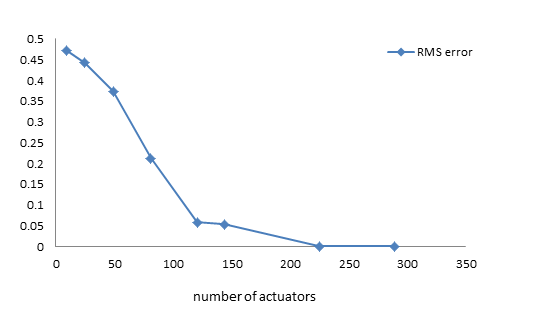
\includegraphics[width=0.7\linewidth]{figures/approx_power}
\caption{Position of actuators (blue) and wavefront samples (red)}.
\label{approx_power}
\end{figure}

\begin{thebibliography}{9}

\bibitem{keck}
  M. A. van Dam, D. L. Mignant, and B. A. Macintosh,
  \emph{Performance of the Keck Observatory adaptive-optics system}.
  Appl. Opt., vol. 43, pp. 5458-5467, Oct 2004

\bibitem{verh}
  M. Verhaegen,
  \emph{Lecture notes for SC4045: Control for High Resolution Imaging}.
  Delft Center for Systems \& Control, TU Delft

\end{thebibliography}

\end{document}
